\section{Prompts} \label{prompts}

This section provides prompts used for Model-as-judge approaches: for numerical estimation of complexity for MASJ in Table~\ref{tab:num_masj_prompt},
for nominal estimation of complexity for MASJ in Table~\ref{tab:nom_masj_prompt},
and for reasoning level estimate in Table~\ref{tab:reasoning_level_prompt}.

\begin{table}[H]
    \small
    \centering
    \caption{Prompt for Numerical model-as-judge}
    \label{tab:num_masj_prompt}
    \begin{tabular}{p{11cm}}
    \hline
    You are an expert in the topic of the question. Please act as an impartial judge and evaluate the complexity of the multiple-choice question with options below. Begin your evaluation by providing a short explanation. Be as objective as possible. After providing your explanation, you must not answer the question. You must rate the question complexity as a number from 0 to 1 following the following scale as a reference: \\
    high\_school\_and\_ easier - 0.0-0.22, \\
    undergraduate\_easy - 0.2-0.4, \\ 
    undergraduate\_hard - 0.4-0.6, \\ 
    graduate - 0.6-0.8, \\ postgraduate - 0.8-1.0. \\
    You must return the complexity by strictly following this format: "  
    [[complexity]]", \\ for example: "Your explanation... Complexity: [[0.55]]", which corresponds to a hard question at the undergraduate level.
    \\
    \hline 
    \end{tabular}
\end{table}

\begin{table}[H]
    \small
    \centering
    \caption{Prompt for Nominal model-as-judge}
    \label{tab:nom_masj_prompt}
    \begin{tabular}{p{11cm}}
    \hline
    You are an expert in the topic of the question. Please act as an impartial judge and evaluate the complexity of the multiple-choice question with options below. Begin your evaluation by providing a short explanation. Be as objective as possible. After providing your explanation, you must not answer the question. You must rate the question complexity by strictly following the scale: \\
    high\_school\_and\_easier, \\ 
    undergraduate\_easy, \\ 
    undergraduate\_hard, \\ 
    graduate, \\ 
    postgraduate. \\
    You must return the complexity by strictly following this format: "[[complexity]]", \\ 
    for example: "Your explanation... Complexity: [[undergraduate]]", which corresponds to the undergraduate level.
    \\
    \hline 
    \end{tabular}
\end{table}

\begin{table}[H]
    \centering
    \small
    \caption{Prompt for Reasoning level estimate}
    \label{tab:reasoning_level_prompt}
    \begin{tabular}{p{11cm}}
    \hline
    You are an expert in the topic of the question. Please act as an impartial judge and evaluate the complexity of the multiple-choice question with options below. \\
    Begin your evaluation by providing a short explanation. Be as objective as possible. After providing your explanation, you must not answer the question. \\
    You must rate the question complexity by strictly following the criteria: \\
    1) [[Requires knowledge]] - do we need highly specific knowledge from the domain to answer this question? Valid answers: yes, no; \\
    2) [[Requires reasoning]] - do we need complex reasoning with multiple logical steps to answer this question? Valid answers: yes, no; \\
    3) [[Number of reasoning steps]] - how many reasoning steps do you need to answer this question? Valid answers: low, medium, high. \\
    Your answer must strictly follow this format:  
    "[[Requires knowledge: answer]] [[Requires reasoning: answer]] [[Number of reasoning steps: answer]]". \\
    Example 1: "Your explanation... [[Requires knowledge: yes]] [[Requires reasoning: no]] [[Number of reasoning steps: low]]". \\
    Example 2: "Your explanation... [[Requires knowledge: no]] [[Requires reasoning: yes]] [[Number of reasoning steps: high]]". \\
    Example 3: "Your explanation... [[Requires knowledge: yes]] [[Requires reasoning: yes]] [[Number of reasoning steps: medium]]". \\
    Example 4: "Your explanation... [[Requires knowledge: no]] [[Requires reasoning: no]] [[Number of reasoning steps: low]]". \\
    \hline
    \end{tabular}
\end{table}

\section{Question examples with answers}
\label{sec:question_examples}

This section provides examples of questions included in the MMLU-Pro dataset on Law, Psychology, and Engineering in Tables~\ref{tab:law_example}, \ref{tab:psychology_example}, and~\ref{tab:engineering_example}, correspondingly. 

\begin{table}[H]
    \small
    \centering
    \caption{Example of a question from Law category}
    \label{tab:law_example}
    \begin{tabular}{p{11cm}}
    \hline
    Which of the following criticisms of Llewellyn's distinction between the grand and formal styles of legal reasoning is the most compelling? \\
    1. There is no distinction between the two forms of legal reasoning. \\
    2. Judges are appointed to interpret the law, not to make it. \\
    3. It is misleading to pigeon-hole judges in this way. \\
    4. Judicial reasoning is always formal. \\
    \hline
    \end{tabular}
\end{table}

\begin{table}[H]
    \small
    \centering
    \caption{Example of a question from Psychology category}
    \label{tab:psychology_example}
    \begin{tabular}{p{11cm}}
    \hline
    A 66-year-old client who is depressed, has rhythmic hand movements, and has a flattened affect is probably suffering from: \\
    1. Huntington's disease \\
    2. Creutzfeldt-Jakob disease \\
    3. Multiple Sclerosis \\
    4. Alzheimer's disease \\
    5. Parkinson's disease \\
    6. Vascular Dementia \\
    7. Frontotemporal Dementia \\
    8. Schizophrenia \\
    9. A right frontal lobe tumor \\
    10. Bipolar Disorder \\
    \hline
    \end{tabular}
\end{table}

\begin{table}[H]
    \small
    \centering
    \caption{Example of a question from Engineering category}
    \label{tab:engineering_example}
    \begin{tabular}{p{11cm}}
    \hline
    A cumulative compound motor has a varying load upon it which requires a variation in armature current from 50 amp to 100 amp. \\
    If the series-field current causes the air-gap flux to change by 3 percent for each 10 amp of armature current, find the ratio of torques developed for the two values of armature current. \\
    1. 2.26 \\
    2. 0.66 \\
    3. 3.95 \\
    4. 1.00 \\
    5. 2.89 \\
    6. 1.75 \\
    7. 4.12 \\
    8. 1.15 \\
    9. 0.87 \\
    10. 3.40 \\
    \hline
    \end{tabular}
\end{table}

\section{Entropy Distributions}
\label{sec:entropy_distributions }

\begin{figure}[H]
\centering
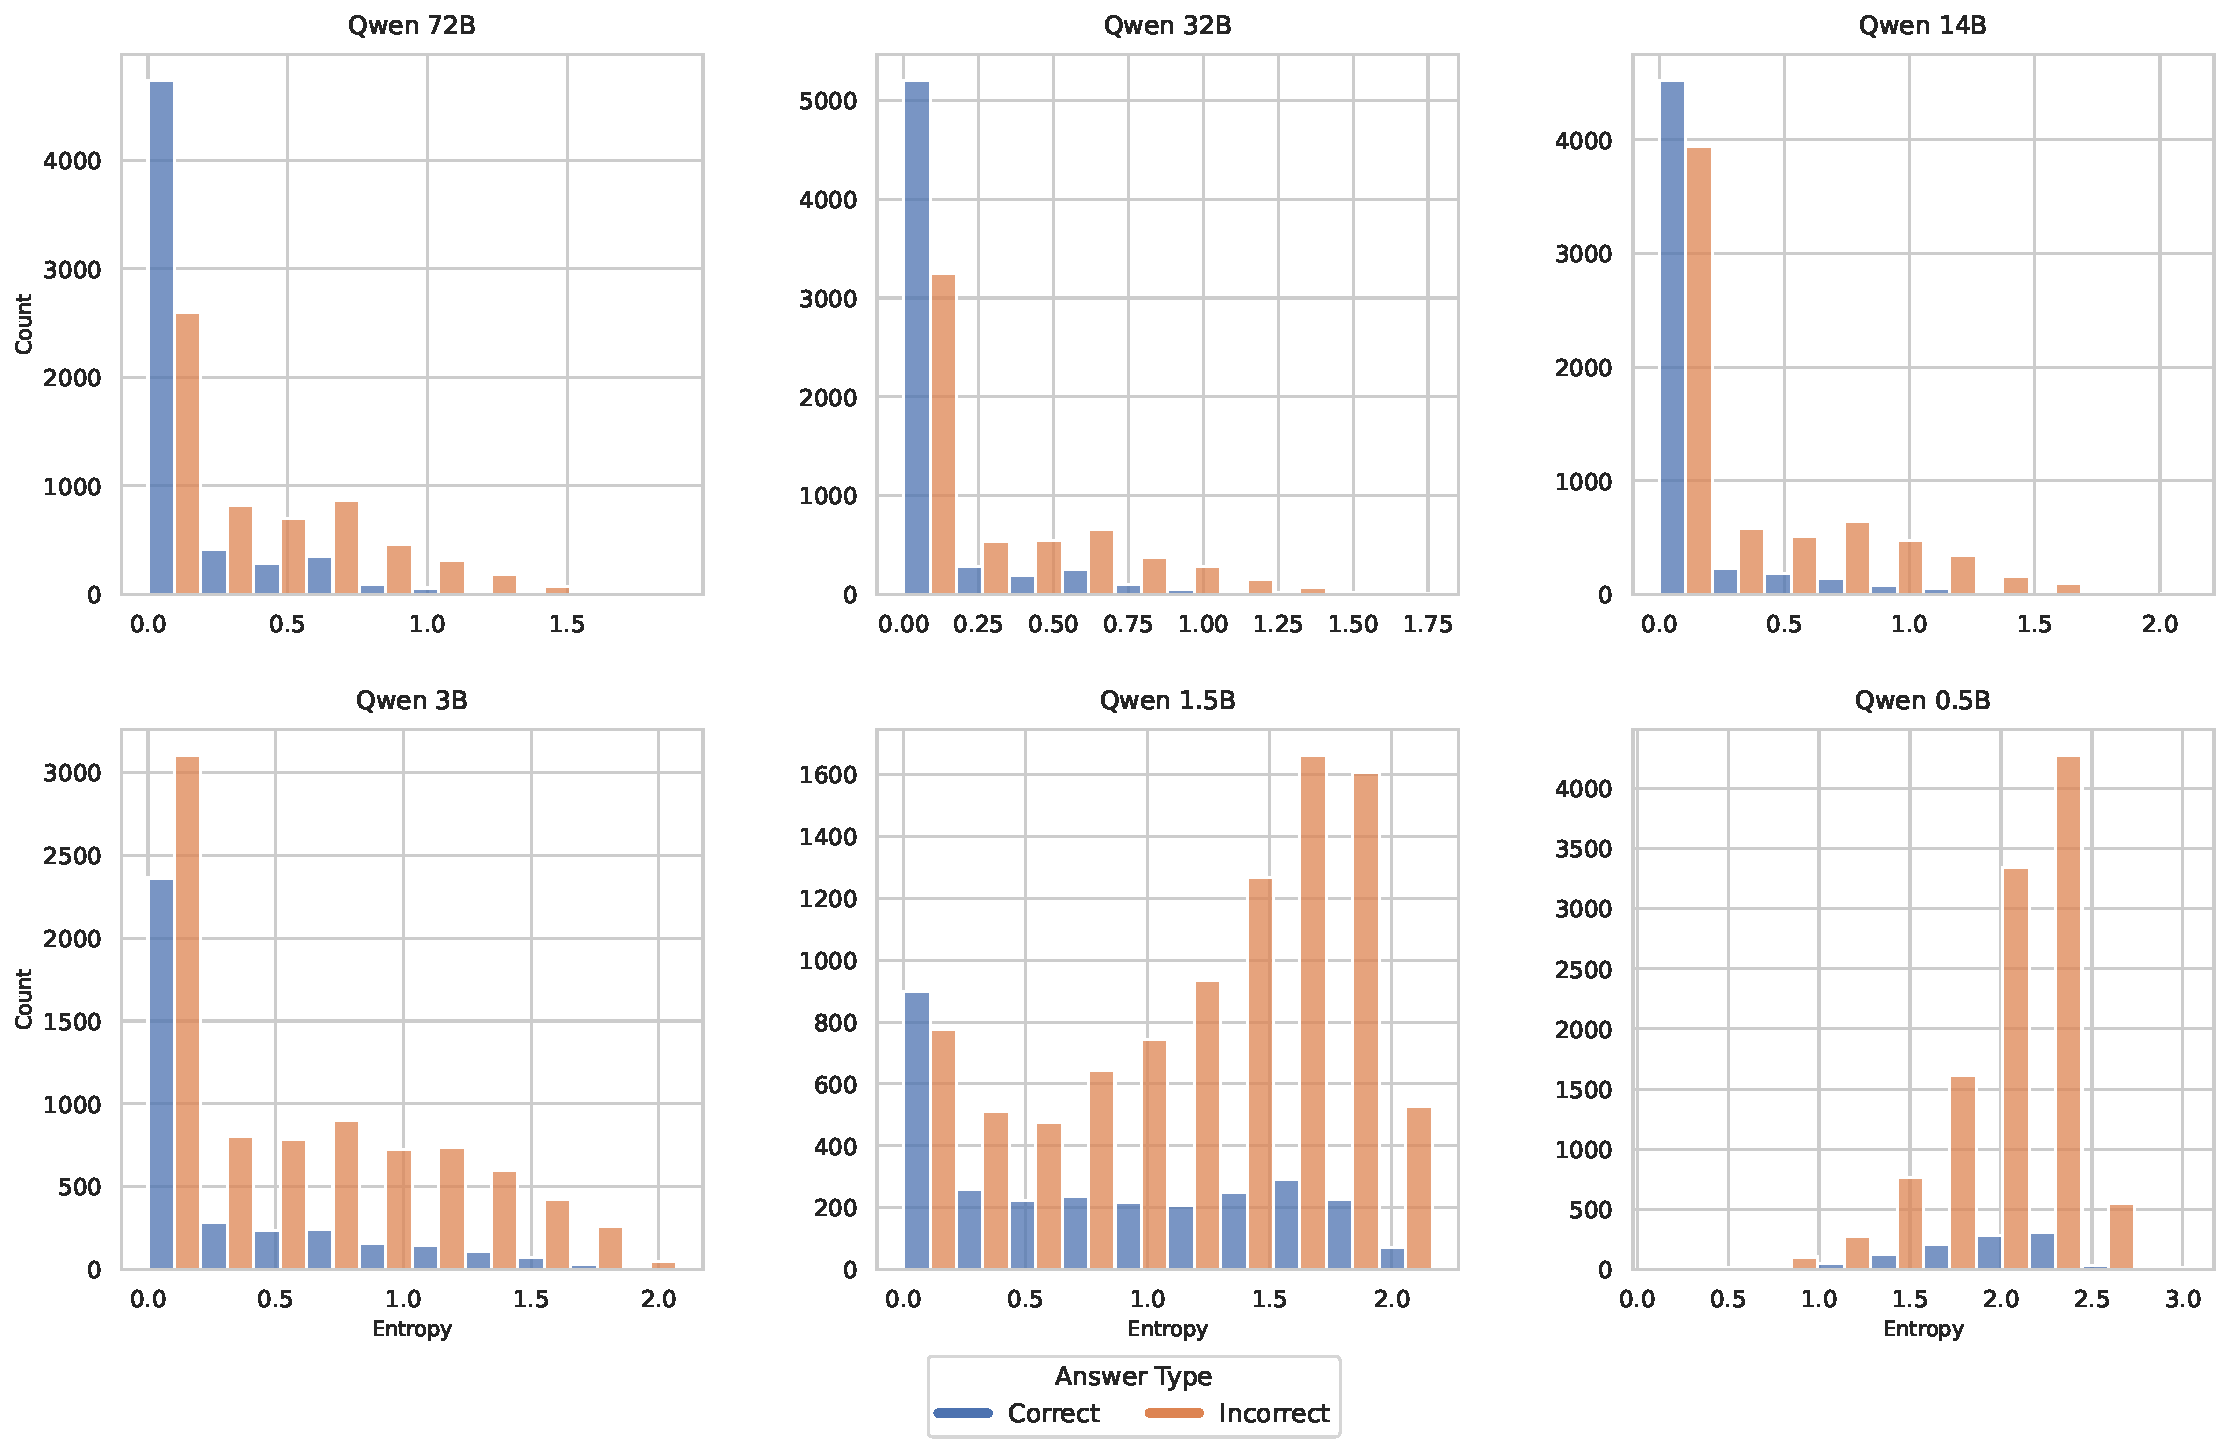
\includegraphics[width=0.95\textwidth]{images/all_models_entropy_counts.pdf}
\caption{Distribution of entropy values for Qwen models (72B, 32B, 14B, 3B, 1.5B, 0.5B), stratified by answer correctness. For larger models (72B, 32B), correct answers (blue) exhibit a pronounced left skew toward low entropy, indicating higher confidence in accurate predictions. Smaller models (1.5B, 0.5B) show flatter distributions, with less separation between correct and incorrect (orange) entropy values. Notably, the 72B variant demonstrates near-zero entropy peaks for correct responses, aligning with findings from Section 4.2.} 
\label{fig:entropy_distributions }
\end{figure}

This section complements the analysis in Section 4.3 by providing full entropy distributions for the Qwen model family. Figure~\ref{fig:entropy_distributions } reveals two key trends:

Model scale correlates with entropy separation: Larger models (72B, 32B) show clearer divergence between correct (low entropy) and incorrect (higher entropy) predictions, while smaller variants (3B, 0.5B) exhibit overlapping distributions.
